%!TEX root = ms.tex
\section{AICc-hdf for BS with orthogonal \texorpdfstring{$X$}{Lg}}
\label{sec:aicc_hdf}
\subsection{A heuristic degrees of freedom for BS}
The edf of BS has an analytical expression only when the true model is $\mu=0$ \citep{Ye1998}. \citet{Tibshirani2015} studied the Lagrangian formulation of BS (LBS) and provided an analytical expression for edf without any restrictions on $\mu$. To distinguish between the two methods, we use df$_C(k)$ and df$_L(\lambda)$ to denote edf of BS for subset size $k$ and edf of LBS for tuning parameter $\lambda$, respectively. In this section, we introduce a heuristic degrees of freedom (hdf) for BS that is built upon the connection between df$_C(k)$ and df$_L(\lambda)$.

\subsubsection{Lagrangian BS and its edf}
For each regularization parameter $\lambda \ge 0$, LBS solves
\begin{equation}
	\min_\beta \frac{1}{2} \lVert \mathbf{y}-\mathbf{X\beta}\rVert_2^2 + \lambda\lVert \mathbf{\beta} \rVert_0.
\label{eq:lbestsubset-setup}
\end{equation} 
Both LBS \eqref{eq:lbestsubset-setup} and BS \eqref{eq:bestsubset-setup} are LS regressions of $y$ upon a certain subset of $X$. With orthogonal $X$, both problems have analytical solutions: $\hat{\beta}_i(\lambda)=z_i \mathbbm{1}_{(|z_{i}| \ge \sqrt{2\lambda})}$ for \eqref{eq:lbestsubset-setup} and $\hat{\beta}_i(k)=z_i \mathbbm{1}_{(|z_{i}| \ge |z_{(k)}|)}$ for \eqref{eq:bestsubset-setup}, where $z=X^T y$ and $z_{(k)}$ is the $k$-th largest coefficient in absolute value. These two problems are not equivalent, and there is no clear one-to-one correspondence between $\lambda$ in \eqref{eq:lbestsubset-setup} and $k$ in \eqref{eq:bestsubset-setup}. Indeed, for each $\lambda$ there exists a $k$ such that $\hat{\beta}(\lambda) = \hat{\beta}(k)$ where $\hat{\beta}(\lambda)$ is the solution of \eqref{eq:lbestsubset-setup} at $\lambda$ and $\hat{\beta}(k)$ is the solution of \eqref{eq:bestsubset-setup} at $k$, but the reverse does not necessarily hold, since there will be multiple $\lambda$ corresponding to the same solution $\hat{\beta}(k)$. Moreover, with a general $X$, solving \eqref{eq:lbestsubset-setup} does not guarantee recovery of the entire solution path given by solving \eqref{eq:bestsubset-setup} for $k=0,\dots,p$.

By assuming an orthogonal $X$, \citet{Tibshirani2015} derived an expression for df$_L(\lambda)$ based on definition \eqref{eq:edf},
\begin{equation}
\text{df}_L(\lambda) = E(k_L(\lambda)) + \frac{\sqrt{2\lambda}}{\sigma} \sum_{i=1}^{p} \left[\phi\left(\frac{\sqrt{2\lambda}-(X^T \mu)_i}{\sigma}\right) + \phi\left(\frac{-\sqrt{2\lambda}-(X^T \mu)_i}{\sigma}\right) \right],
\label{eq:thdf_expression}
\end{equation}
where the expected subset size is given as
\begin{equation}
E(k_L(\lambda)) = \sum_{i=1}^{p} \left[1-\Phi\left(\frac{\sqrt{2\lambda}-(X^T \mu)_i}{\sigma}\right) + \Phi\left(\frac{-\sqrt{2\lambda}-(X^T \mu)_i}{\sigma}\right) \right].
\label{eq:thdf_size_expression}
\end{equation}

\subsubsection{hdf for BS}
Given the similarity of problems \eqref{eq:bestsubset-setup} and \eqref{eq:lbestsubset-setup}, we would like to approximate df$_C(k)$ with df$_L(\lambda)$. One implementation of this proceeds as follows. Note that df$_C(k)$ is a discrete function of $k=0,\cdots,p$ while df$_L(\lambda)$ is a continuous function of a real variable $\lambda\ge 0$. We propose an hdf that uses $\text{df}_L(\lambda)$ for a particular value of $\lambda$ depending on $k$ as a proxy for $\text{df}_C(k)$. Based on \eqref{eq:thdf_size_expression}, $\lambda$ and $E(k_L(\lambda))$ have a clear one-to-one correspondence, which implies that we can find a unique $\lambda_k^\star$ such that $E(k_L(\lambda_k^\star)) = k$ for each $k=1,\cdots,p$. The value of hdf is df$_L(\lambda_k^\star)$ obtained by substituting $\lambda^\star_k$ into \eqref{eq:thdf_expression}. We also let hdf$(0)=0$ since df$_C(0)=0$. The implementation process is summarized in Algorithm \ref{alg:hdf}. Note that hdf requires estimates of $\mu$ and $\sigma$, and we use the estimates from the LS regression on all predictors. 

% algorithm of hdf
\begin{algorithm}
	\caption{The heuristic df (hdf) of BS for size $k$}\label{alg:hdf}
	Input: $X$ (orthogonal), $\sigma$ and $\mu$. For a given subset size $k$, 
	\begin{enumerate}[label=\arabic*.]
		\item Based on \eqref{eq:thdf_size_expression}, calculate $\lambda_k^\star$ such that $E(k_L(\lambda_k^\star)) = k$.
		\item Based on \eqref{eq:thdf_expression}, calculate hdf$(k) = \text{df}_L(\lambda_k^\star)$.
	\end{enumerate}
	Repeat the above steps for $k=1,\cdots,p$ and let hdf$(0)=0$, yielding hdf for each subset. 
	
	In place of $\mu$ and $\sigma$ in \eqref{eq:thdf_expression} and \eqref{eq:thdf_size_expression}, we use OLS estimates based on the full model, i.e. $\hat{\mu}=XX^T y$, $\hat{\sigma}^2 = \lVert y-\hat{\mu} \rVert_2^2/(n-p)$.
\end{algorithm}

\subsubsection{Theoretical justification of hdf under a null true model}
Assume $\mu=0$, with $X$ still being orthogonal. In such a restricted scenario, df$_C(k)$ has an analytical expression, which allows us to provide some theoretical justification for hdf$(k)$. We start by introducing notation, and present the main result in Theorem \ref{thm:hdf_ydf_representation} and its Corollary. The detailed proofs are given in the Supplemental Material.

Denote $\tilde{X}_{(i)}$ as the $i$-th largest order statistic in an i.i.d sample of size $p$ from a $\chi^2_1$ distribution. \citet{Ye1998} showed that
\begin{equation*}
\text{df}_C(k) = E\left( \sum_{i=1}^{k} \tilde{X}_{(i)} \right).
\end{equation*}
Let $\tilde{H}(s) = -\tilde{Q}(1-s)$ where $\tilde{Q}$ is the quantile function of a $\chi_1^2$ distribution, and $s\in (0,1)$. For $0\le s \le t \le 1$, the truncated variance function is defined as
\begin{equation*}
\tilde{\sigma}^2(s,t) = \int_{s}^{t} \int_{s}^{t} (u \wedge v -uv) d \tilde{H}(u) d \tilde{H}(v),
\end{equation*}
where $u \wedge v =\min(u,v)$. Denote $\tilde{Y}_p = \tilde{\sigma}_p^{-1}(\sum_{i=1}^k \tilde{X}_{(i)} - \tilde{\mu}_p)$, where
\begin{equation*}
\tilde{\sigma}_p = \sqrt{p} \cdot \tilde{\sigma}(1/p,k/p),
\end{equation*}
and
\begin{equation*}
\tilde{\mu}_p = -p \int_{1/p}^{k/p} \tilde{H}(u) du - \tilde{H}\left(\frac{1}{p}\right).
\end{equation*}

\begin{restatable}{theorem}{dfasy}
	\label{thm:hdf_ydf_representation}
	Assume $X$ is orthogonal and the true model is null ($\mu=0$). As $p\rightarrow  \infty$,  $k\rightarrow  \infty$ with $k=\left \lfloor{px}\right \rfloor$, we have
	\begin{equation}
	\label{eq:hdf_ydf_yp_representation}
	\frac{1}{2p} \text{hdf}(k) = \frac{1}{2p}\text{df}_C(k) - \frac{\tilde{\sigma}_p}{2p}E(\tilde{Y}_p) + O\left(\frac{\log(p)}{p} \right),
	\end{equation}
	where $x \in (0,1)$ is a constant and $\left \lfloor{\cdot}\right \rfloor$ denotes the greatest integer function.
\end{restatable}

\begin{restatable}{corollary}{dfasycorollary}
	\label{thm:hdf_ydf_corollary}
	If $\limsup |E(\tilde{Y}_p)| < \infty$ , we further have
	\begin{equation}
	\label{eq:main_corollary}
	\frac{\text{df}_C(k)}{\text{hdf}(k)} \rightarrow 1.
	\end{equation}
\end{restatable}
\noindent\textbf{Remark:} If $\tilde{Y}_p$ is uniformly integrable, then $E(\tilde{Y}_p) \rightarrow 0$, and hence the result of Corollary \ref{thm:hdf_ydf_corollary} holds.

It can be seen that Corollary \ref{thm:hdf_ydf_corollary} holds given the assumptions, since both hdf$(k)$ and df$_C(k)$ diverge while $E(\tilde{Y}_p)$ and the remainder term remain bounded. The Corollary suggests that for large $k$ and large $p$, the ratio of df$_C(k)$ to hdf$(k)$ will be close to $1$. We next explore empirically the relative behavior of the two dfs for a fixed $p$ with an increasing $k$. 

\subsubsection{Numerical justification of hdf}
Figure \ref{fig:dfc_dflambda} shows the comparison of hdf and edf via simulations. We fit BS on $1000$ realizations of the response generated after fixing $X$. The edf is calculated based on definition \eqref{eq:edf} using the sample covariances, while hdf is given by Algorithm \ref{alg:hdf}. We see that in the null case, using hdf to approximate edf becomes more accurate as $k$ approaches $p$, providing a finite-sample justification of Corollary \ref{thm:hdf_ydf_corollary}. 

In addition to the null model, we consider a sparse model (Orth-Sparse-Ex1) with $p_0=6$ true predictors (those with non-zero coefficients), and a dense model (Orth-Dense) where all predictors have non-zero coefficients. We also consider two signal-to-noise (SNR) ratios with ``hsnr'' and ``lsnr'' representing high and low SNR respectively, and the SNR is defined as $\text{Var}(x^T \beta)/\sigma^2$. The details of the setups for Orth-Sparse-Ex1 and Orth-Dense models can be found in Section \ref{sec:simulation_setup_orthx}. Similarly to the null case, we see that hdf approaches edf as $k$ gets close to $p$, i.e. the statement of Corollary \ref{thm:hdf_ydf_corollary} holds in these scenarios as well. Furthermore, we see that hdf generally approximates edf well, where the difference is more pronounced when BS underfits, e.g. a sparse model with high SNR and $k<p_0=6$ or a dense model with high SNR with $k<p=14$. Clearly, underfitting causes the problem, particularly when what is left out is important, such as in a high SNR case.   


% \ref{fig:dfc_dflambda}
\begin{figure}[!ht]
	\centering
	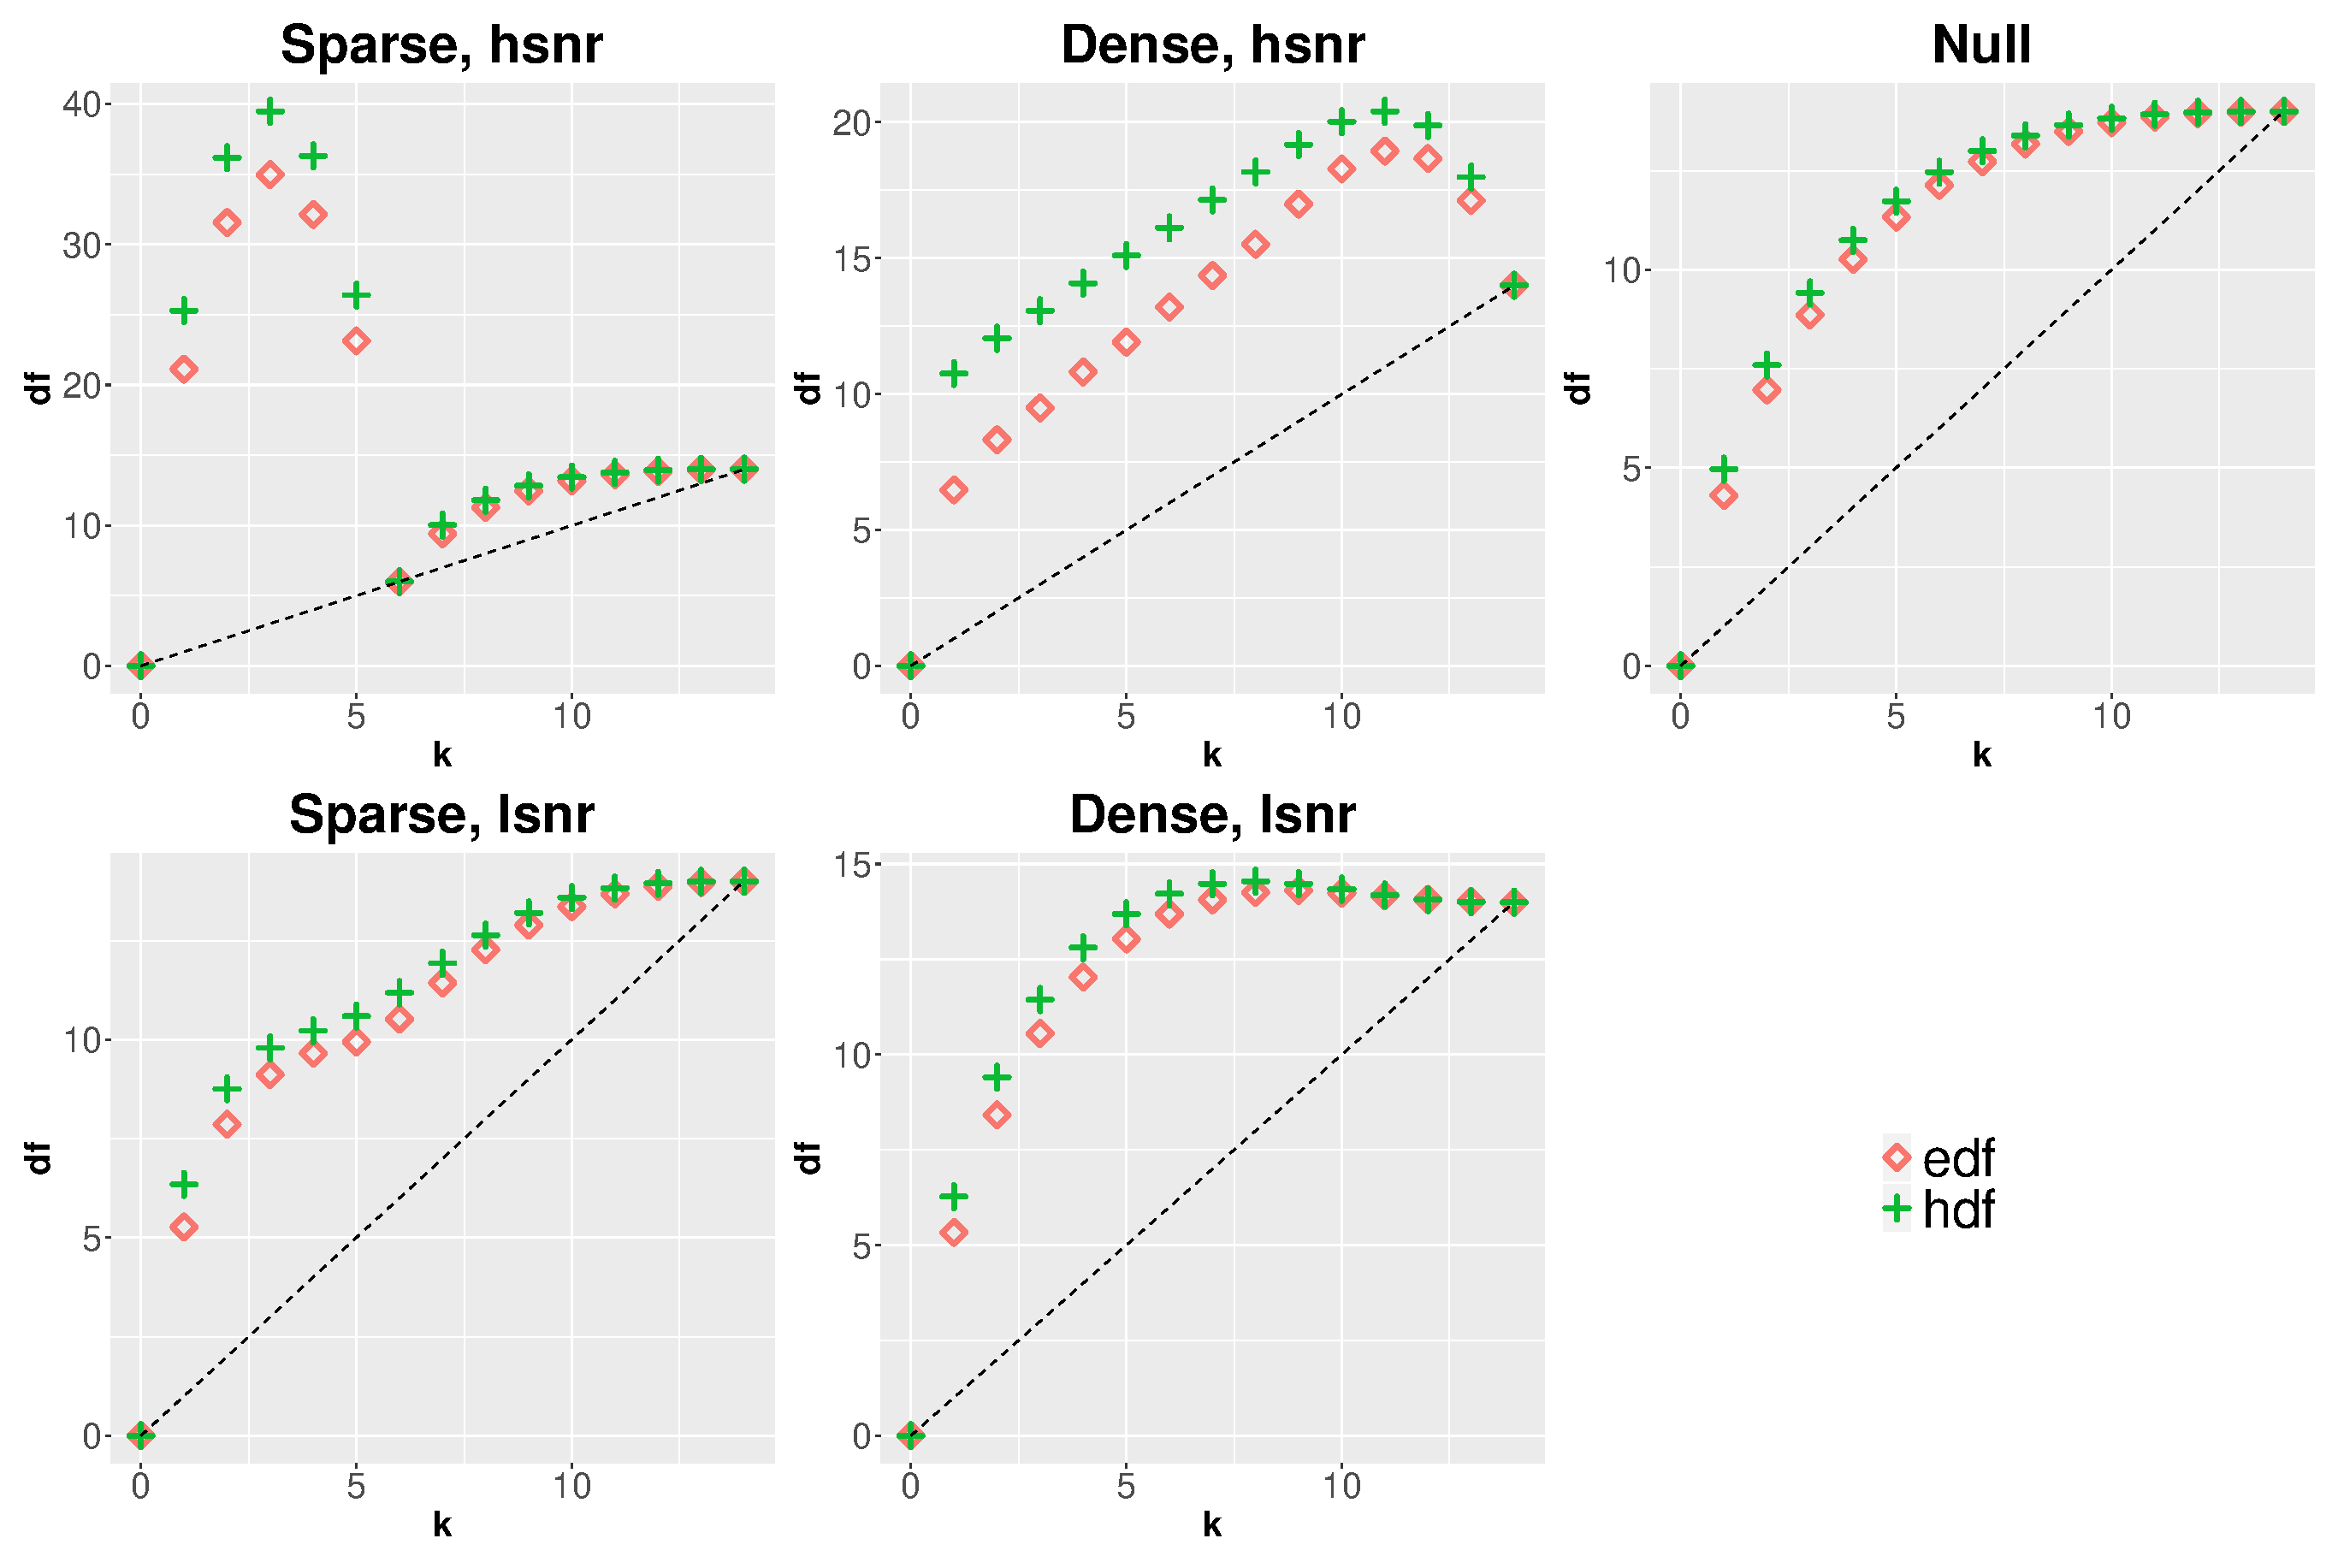
\includegraphics[width=0.9\textwidth]{figures/hdf_edf_bs.eps}
	\caption{hdf$(k)$ and df$_C(k)$ (edf of constrained BS). The black dashed line is the 45-degree line. Here $X$ is orthogonal with $n=200$ and $p=14$. Three types of the true model and two SNR are considered. We assume knowledge of $\mu$ and $\sigma$.}
	\label{fig:dfc_dflambda}
\end{figure}



\subsubsection{\texorpdfstring{C$_p$}{Lg}-hdf as a feasible implementation of \texorpdfstring{C$_p$}{Lg}-edf }
\label{sec:cp_edf_hdf}
We have shown that hdf generally approximates edf well, and it agrees with edf as $k$ approaches $p$. By replacing edf with hdf in \eqref{eq:cp_edf}, we have a feasible selection rule C$_p$-hdf. Figure \ref{fig:cp_edf_hdf} compares the averages of C$_p$-edf and C$_p$-hdf over $1000$ replications. Similarly to the comparison of the degrees of freedom values, we see C$_p$-hdf agrees with C$_p$-edf on average as $k$ approaches $p$. Even at the places where we see differences between the degrees of freedom values, e.g. a sparse true model with high SNR and $k<p_0=6$, the differences are compensated by the model fit and we see C$_p$-hdf is very close to C$_p$-edf. As we discussed in Section \ref{sec:optimism}, for any general fitting procedure including BS, C$_p$-edf provides an unbiased estimator of the expected prediction error where the error measure $\Theta$ is the squared error (SE), i.e. $E(\text{C}_p\text{-edf}) = E(\text{Err}_{\text{SE}})$. Therefore, by using the sample average to represent the population mean, Figure \ref{fig:cp_edf_hdf} indicates that $E(\text{C}_p\text{-hdf})$ approximates $E(\text{Err}_{\text{SE}})$ well, and moreover C$_p$-hdf gives the same average selected size as C$_p$-edf in all cases, when they are applied as selection rules, supporting the use of hdf in model selection for BS.

% \ref{fig:cp_edf_hdf} 
\begin{figure}[!ht]
	\centering
	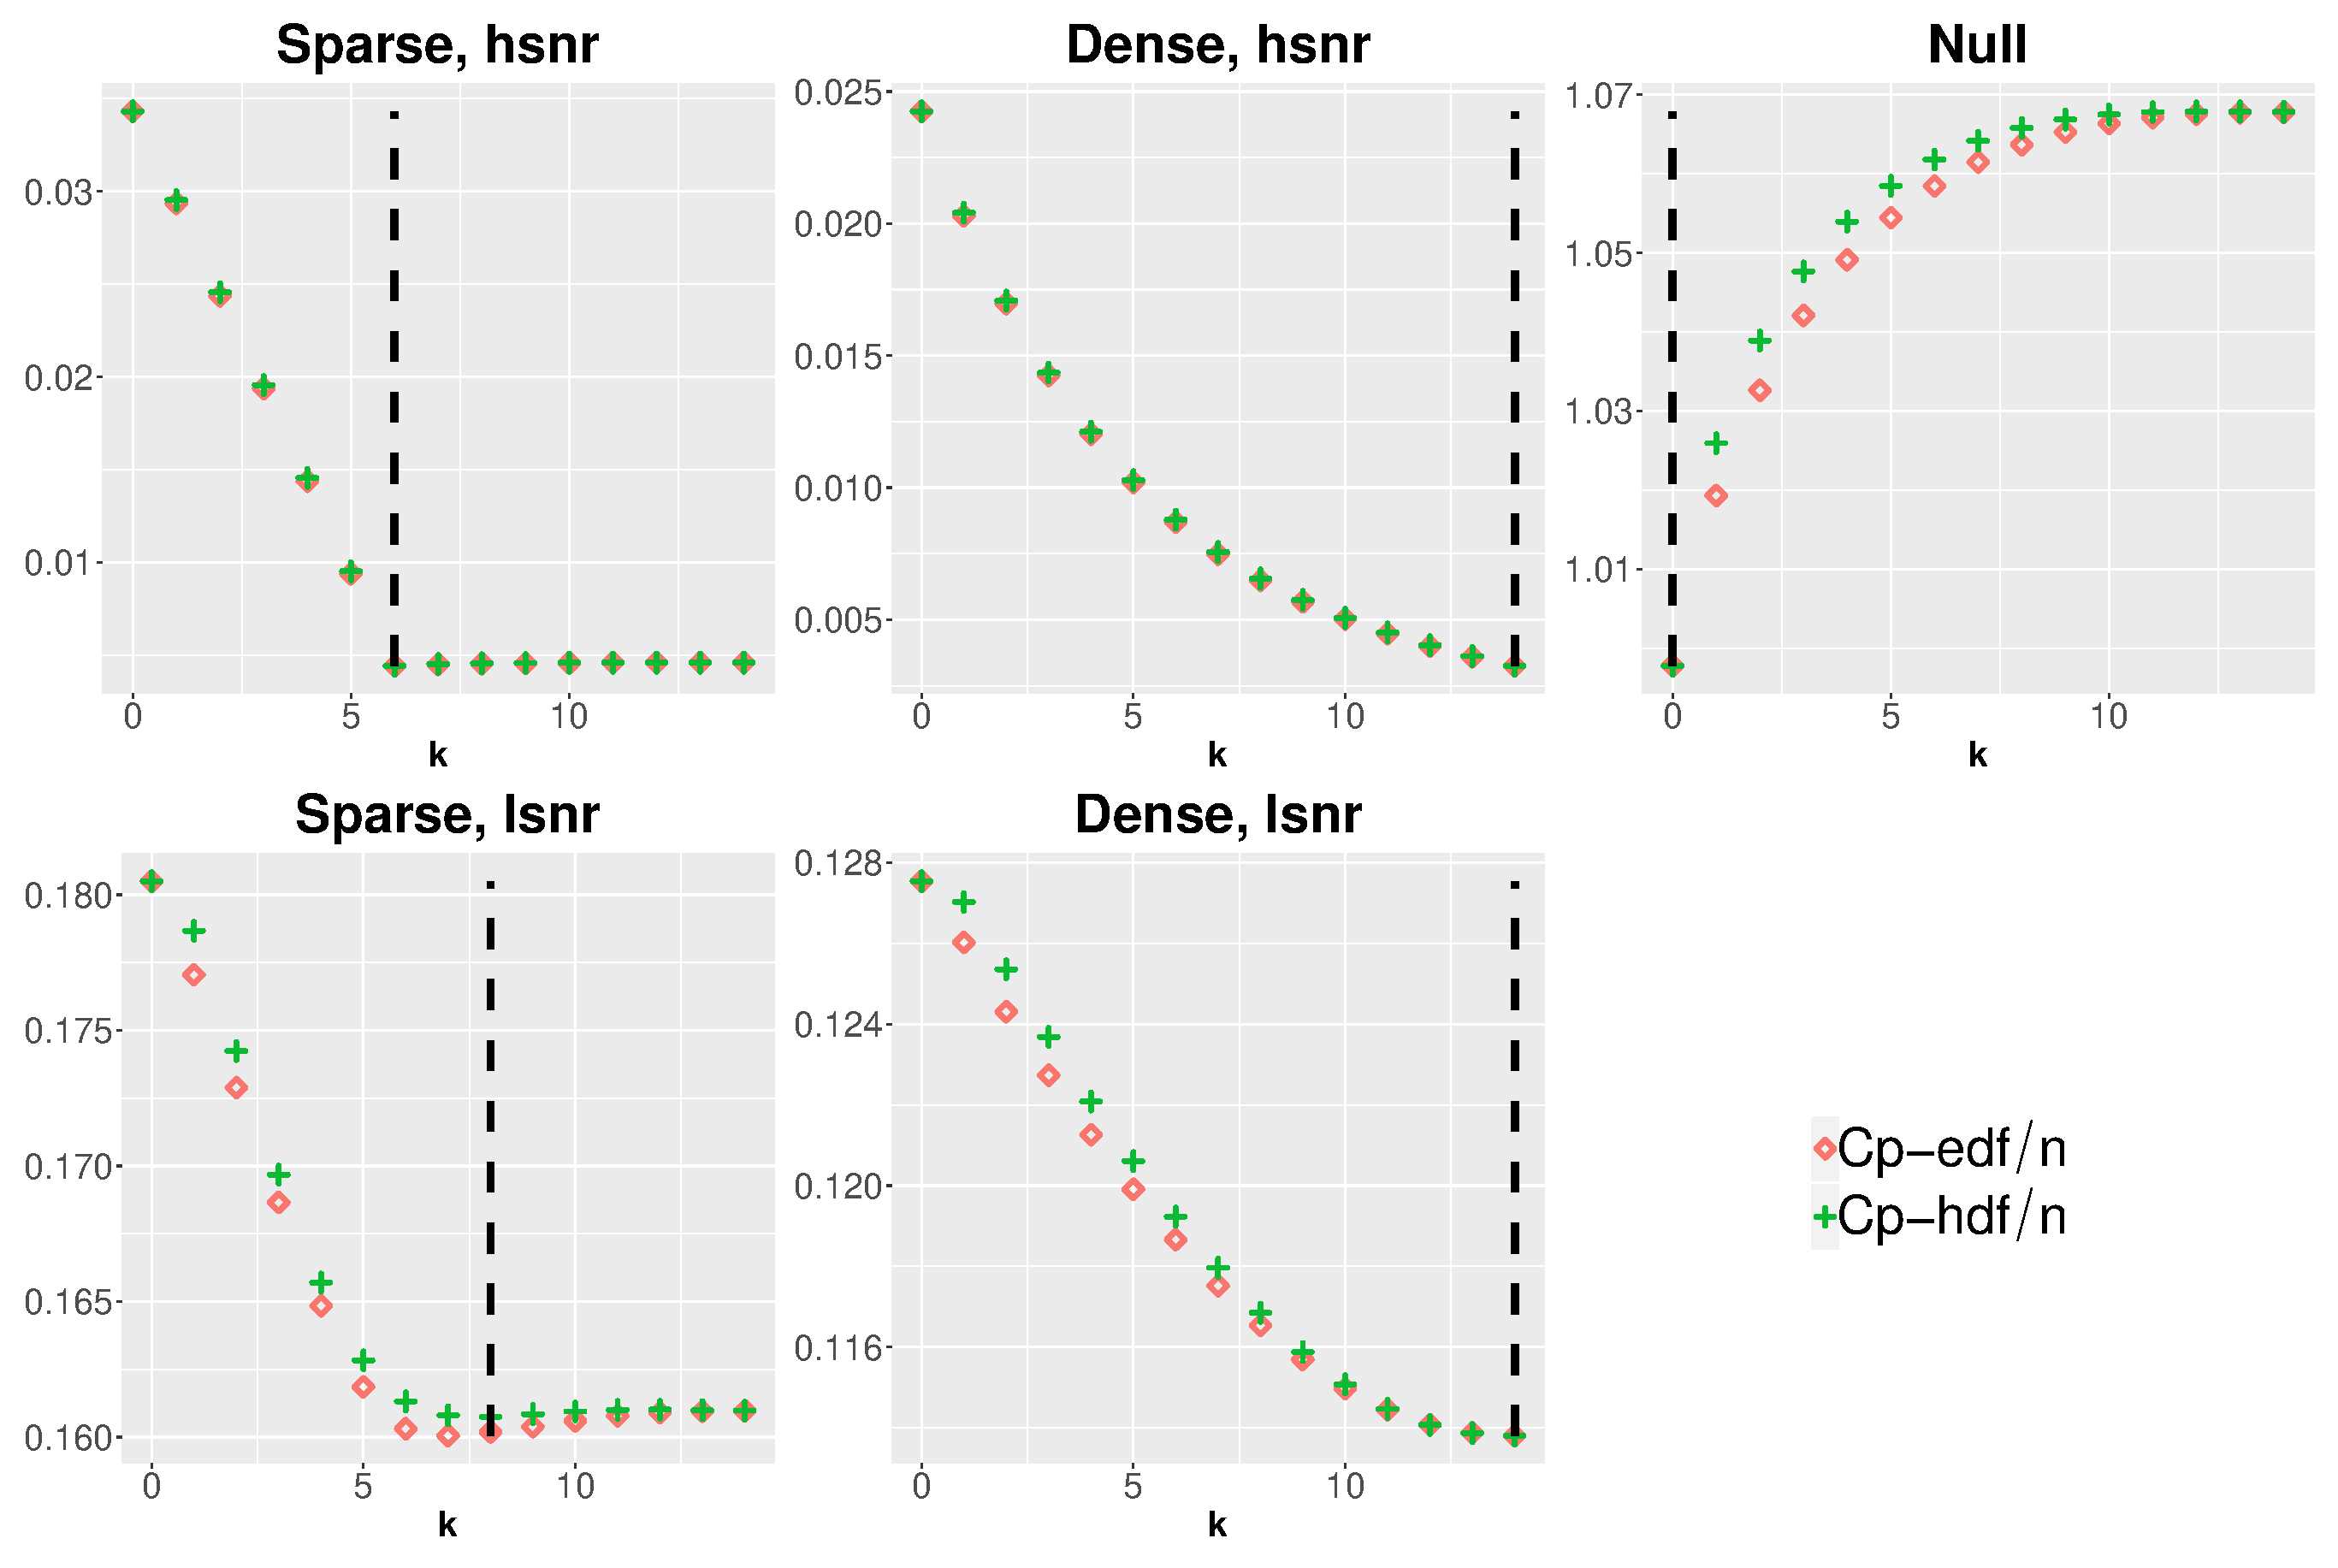
\includegraphics[width=0.9\textwidth]{figures/cp_edf_hdf_bs.eps}
	\caption{Averages of C$_p$-edf and C$_p$-hdf over $1000$ replications. Both criteria lead to the same average of the selected subset size over the $1000$ replications (rounded to the nearest integer), as denoted by the black dashed vertical lines. Other details are the same as in Figure \ref{fig:dfc_dflambda}.}
	\label{fig:cp_edf_hdf} 
\end{figure}


\subsection{A KL-based information criterion for BS}
When the error measure $\Theta$ is the deviance \eqref{eq:deviance_def}, the prediction error $\text{Err}_\text{KL}$ is the KL discrepancy. AICc-edf \eqref{eq:aicc_edf} is motivated by trying to construct an unbiased estimator of $E(\text{Err}_\text{KL})$. The expected KL-based optimism for BS is given as
\begin{equation}
E(\text{op}_\text{KL}) = E\left(n \frac{n\sigma^2+\lVert \mu-X\hat{\beta}(k) \rVert_2^2}{\lVert y-X\hat{\beta}(k)\rVert_2^2}\right) + n.
\label{eq:eop_expression}
\end{equation}
Note that \eqref{eq:eop_expression} holds for a general $X$. Augmenting $E(\text{op}_\text{KL})$ with the training error $\text{err}_{\text{KL}}$ we have $\widehat{\text{Err}}_{\text{KL}}$ according to \eqref{eq:err_eop}, where (ignoring the constant $n\log(2\pi)$ for convenience)
\begin{equation}
\text{err}_{\text{KL}} = n\log\left(\frac{\text{RSS}}{n}\right) - n,
\label{eq:err_expression}
\end{equation}
since the pre-specified model $f$ in \eqref{eq:deviance_def} follows a Gaussian distribution as assumed in \eqref{eq:truemodel_def}. The derivations of \eqref{eq:eop_expression} and \eqref{eq:err_expression} are presented in the Supplemental Material. 

Figure \ref{fig:eop_approx_withrss} shows the averages of AICc-edf, AICc-hdf (AICc-hdf is calculated by replacing edf with hdf in \eqref{eq:aicc_edf}) and $\widehat{\text{Err}}_{\text{KL}}$ over $1000$ replications. By using the sample average to represent population mean, we first see that $E(\text{AICc-edf})$ generally tracks the expected KL, $E(\text{Err}_{\text{KL}})$ reasonably well. In fact, they agree with each other in the null case and a sparse true model with high SNR. Noticeable discrepancies can be observed in a sparse true model with high SNR and $k<p_0=6$. This is the place where the set of true predictors is not entirely included in the model. The derivations of the classic AIC and AICc (both with ndf plugged in according to our notation) are based on an assumption that the true predictors are included in the model. In the situation where this assumption is violated, AICc will no longer be unbiased, and a similar conjecture can be made here for AICc-edf in the context of BS. Second, similarly to the comparison of $E(\text{C}_p\text{-edf})$ and $E(\text{C}_p\text{-hdf})$ in Section \ref{sec:cp_edf_hdf}, we see that $E(\text{AICc-hdf})$ approximates $E(\text{AICc-edf})$ well and they agree with each other as $k$ approaches $p$. 
Last and most importantly, both AICc-edf and AICc-hdf yield the same average selected size as $\widehat{\text{Err}}_{\text{KL}}$ across all scenarios, supporting the use of AICc-hdf as a selection rule for BS.

% \ref{fig:eop_approx_withrss} 
\begin{figure}[!ht]
	\centering
	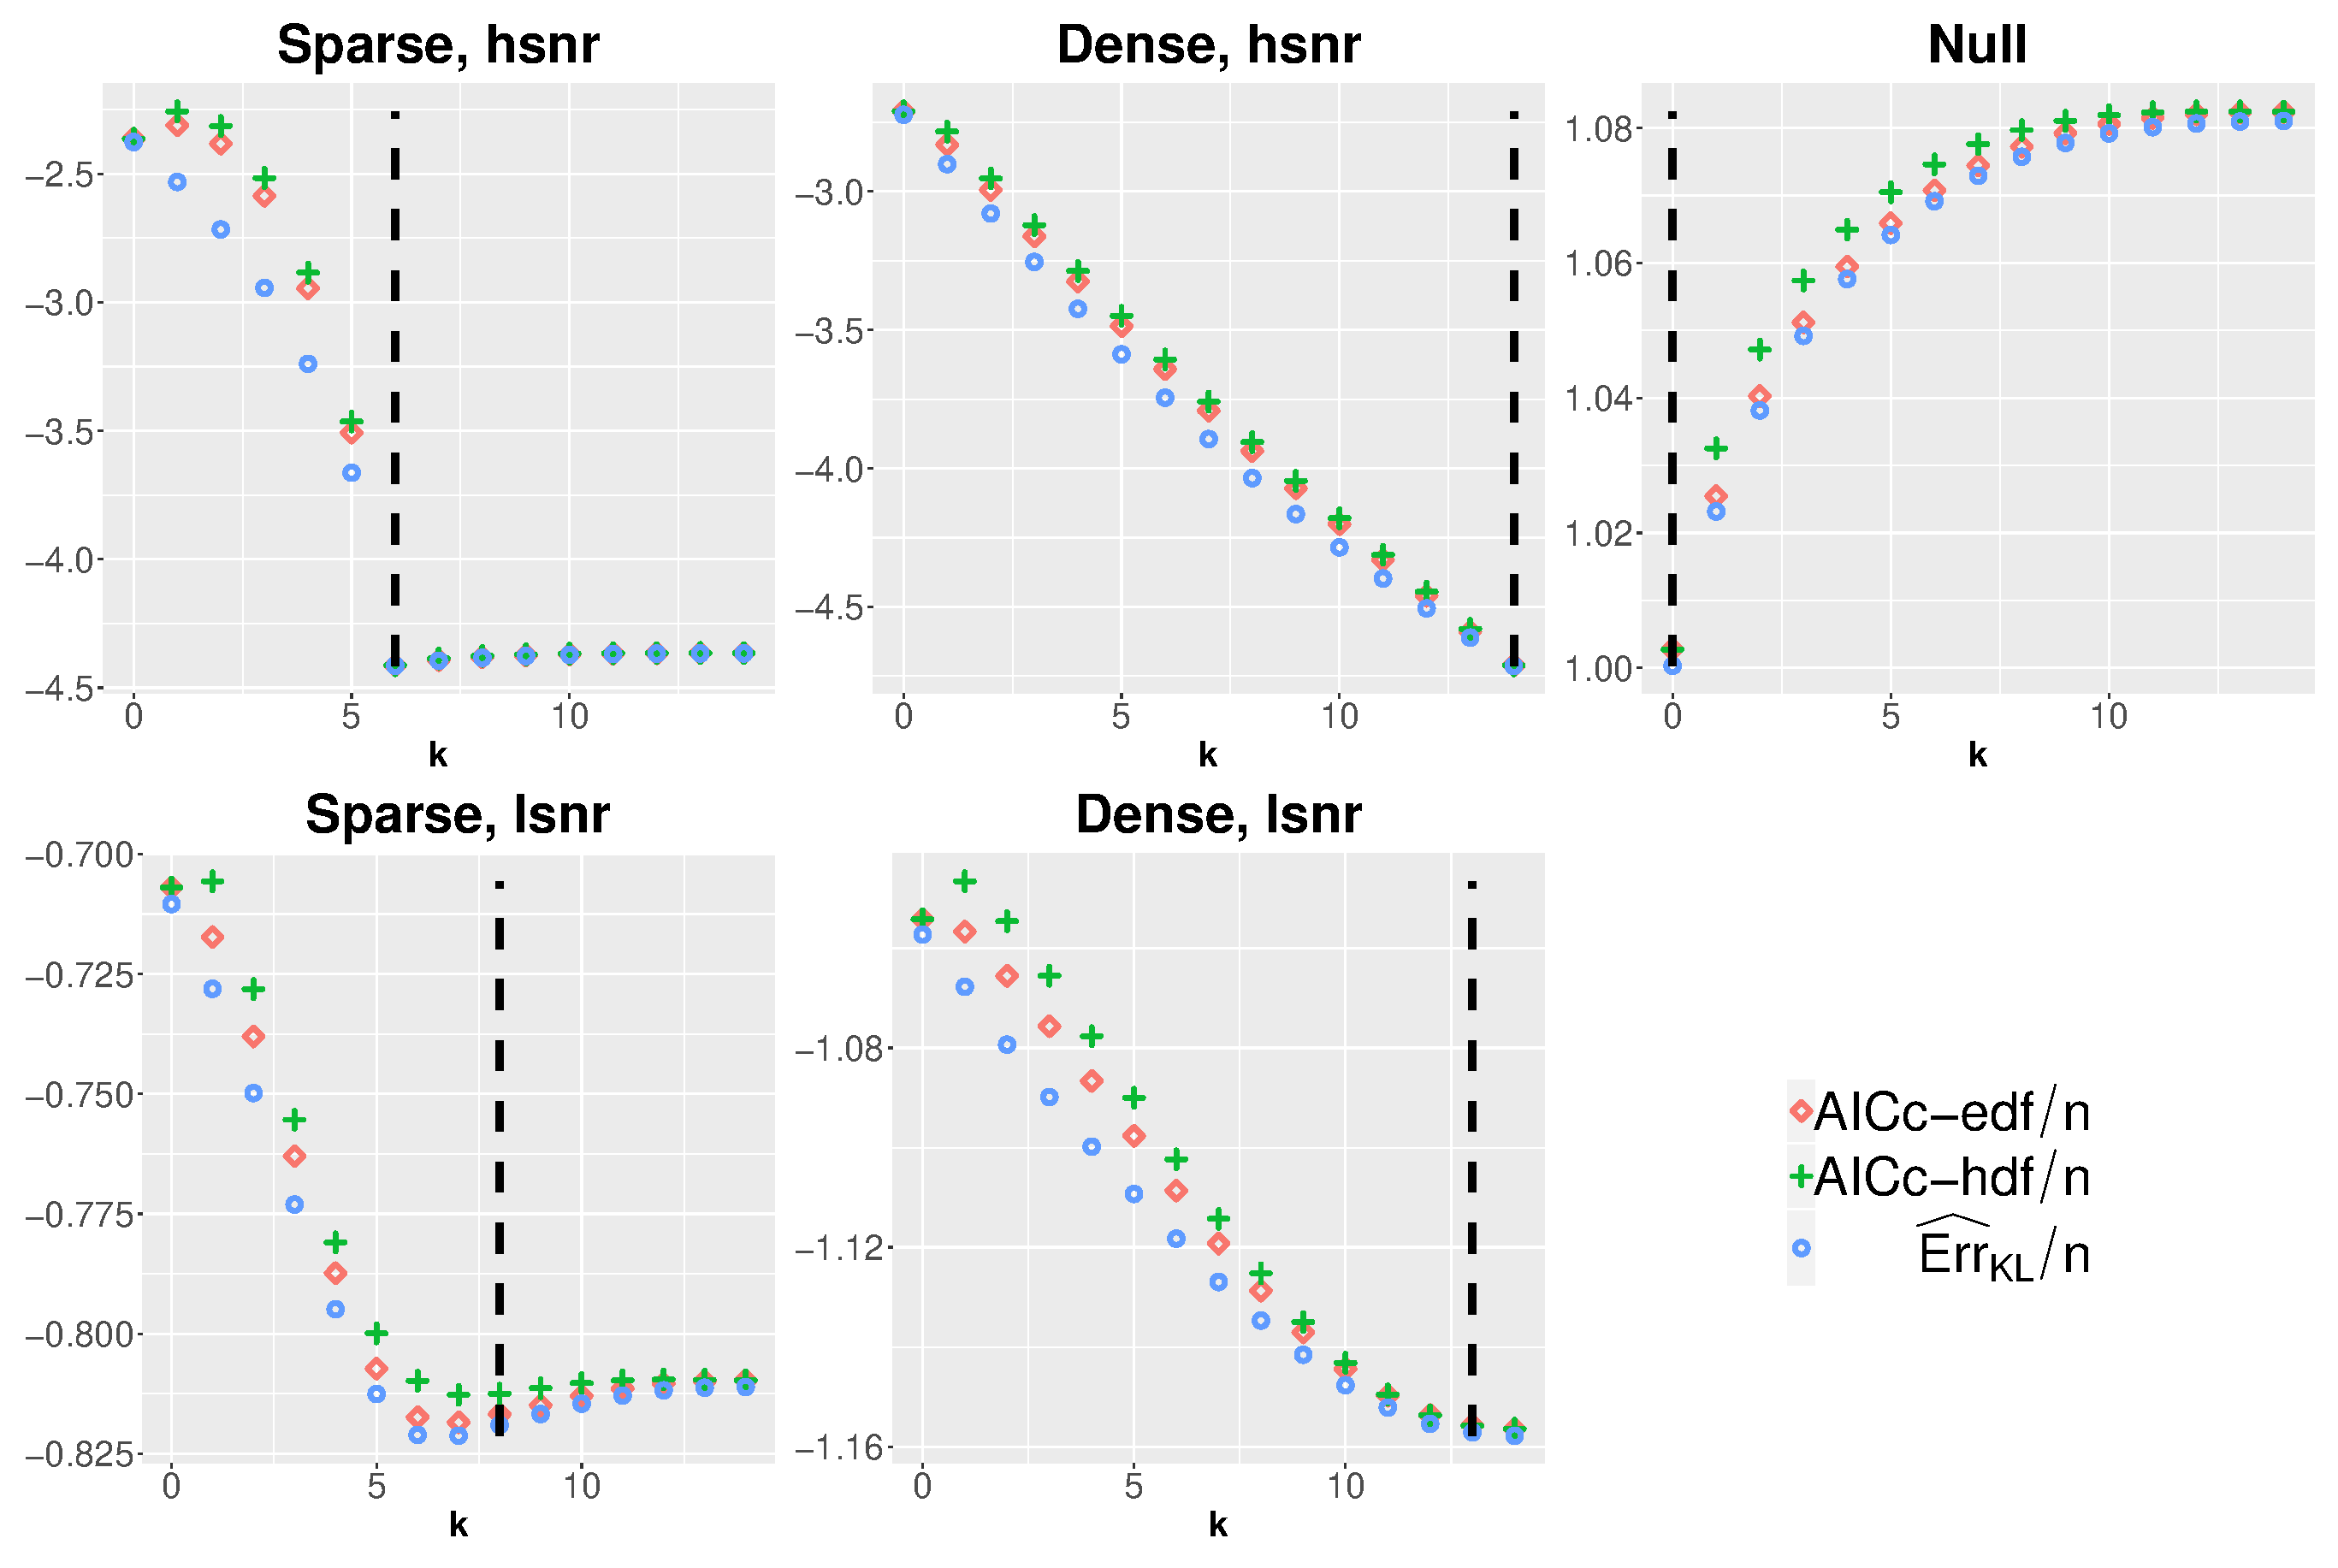
\includegraphics[width=0.9\textwidth]{figures/aicc_edf_hdf_kl_bs.eps}
	\caption{Averages of AICc-edf, AICc-hdf and $\widehat{\text{Err}}_\text{KL}$ over $1000$ replications. All three criteria lead to the same average of the selected subset size over the $1000$ replications (rounded to the nearest integer), as denoted by the black dashed vertical lines. Other details are the same as in Figure \ref{fig:dfc_dflambda}.}
	\label{fig:eop_approx_withrss} 
\end{figure}

\subsection{The performance of AICc-hdf as a selection rule for BS}
We now study the performance of AICc-hdf as a selection rule for BS. The only assumption we make in the simulations is $X$ being orthogonal. Both $\mu$ and $\sigma$ are treated unknown, as would be the case in practice. We start by showing that AICc-hdf can perform well for BS compared to other selection rules. We then compare the performance of BS-AICc-hdf to that of regularization methods. 

\subsubsection{Simulation set-up}
\label{sec:simulation_setup_orthx}
We consider a trigonometric configuration of $X$ that is studied by \citet{Hurvich1991}, where $X=(x^1,x^2)$ is an $n$ by $p$ matrix with components defined by 
$$ x_{tj}^1 = \sin\left(\frac{2\pi j}{n}t\right),$$
and 
$$ x_{tj}^2 = \cos\left(\frac{2\pi j}{n}t\right),$$
for $j=1,\cdots,p/2$ and $t=0,\cdots,n-1$. The columns of $X$ are then standardized to have $l_2$ norm 1, to make them orthonormal. By fixing $X$, the responses are generated by \eqref{eq:truemodel_def}, where $\mu=X\beta$. The error $\epsilon$ is also shifted to have mean $0$, hence the intercept will be zero. 

We consider the following configurations of the experiment:
\begin{itemize}
	\item Sample size: $n \in \{200, 2000\}$.
	\item Number of predictors: $p \in \{14,30,60,180\}$.
	\item Signal-to-noise ratio: $\text{SNR} \in \{0.2,1.5,7\}$ (low, medium and high). The average oracle $R^2$ (linear regression on the set of true predictors) corresponding to these three SNR values are roughly $20\%$, $50\%$ and $90\%$, respectively.
	\item Coefficient vector $\beta$ (Orth in the following denotes for orthogonal $X$):
	\begin{itemize}
		\item Orth-Sparse-Ex1: $\beta=[1_6,0_{p-6}]^T$
		\item Orth-Sparse-Ex2: $\beta=[1,-1,5,-5,10,-10,0_{p-6}]^T$
		\item Orth-Dense \citep{Taddy2017}: $\beta_j = (-1)^j \exp(-\frac{j}{\kappa})$, $j=1,\cdots,p$. $\kappa=10$ 
		%\item Dense-Ex2: same definition of $\beta$ as in Dense-Ex1, but with $\kappa=50$
	\end{itemize}
\end{itemize}

\iffalse
Note that all of the coefficients in the dense designs are non-zero, but many of them have little effects. Dense-Ex1 has a fast decay where only $23$ coefficients have absolute values larger than $0.1$, while the slow decay Dense-Ex2 has $115$ coefficients larger than $0.1$. The dense designs are introduced by \citet{Taddy2017}.
\fi

In total, there are $72$ different scenarios in the experiment. The full set of simulation results is presented in the Supplemental Material. In each scenario, $1000$ replications of the response $y$ are generated. A fitting procedure $\hat{\mu}$, is evaluated via the average RMSE, where 
\begin{equation}
\text{RMSE}(\hat{\mu}) = \sqrt{ \frac{1}{n} \lVert \hat{\mu}-X\beta \rVert_2^2}.
\label{eq:l2_loss}
\end{equation}
To make the scales easier to compare, we construct two relative metrics: $\%$ worse than the best possible BS, and relative efficiency, which are defined as follows:
\begin{itemize}
	\item \textbf{$\%$ worse than best possible BS}
	\begin{equation} 
	=\displaystyle 100 \times \left( \frac{\text{averge RMSE of a fitting procedure } \hat{\mu}}{\text{average RMSE of the best possible BS}} - 1 \right) \%,
	\end{equation}
	where the best possible BS here means that on a single fit, choosing the subset size with the minimum RMSE among all $p+1$ candidates, as if an oracle tells us the true model.
	
	\item \textbf{Relative efficiency:} For a collection of fitting procedures, the relative efficiency for a particular procedure $j$, is defined as
	\begin{equation}
	\displaystyle \frac{\min_l \text{ average RMSE of fitting procedure }l}{\text{average RMSE of fitting procedure }j}.
	\end{equation}
	The relative efficiency is a measure between $0$ and $1$. Higher value indicates better performance. Besides the fitting procedures specified, we include the null and full OLS in the calculation of relative efficiency. 
\end{itemize}
We also present the sparsistency (number of true positives) and number of extra predictors (number of false positives). 


\subsubsection{AICc-hdf and other selection rules for BS}
\label{sec:bs_ic_simulationresults}
By analogy to C$_p$ and AICc, we can also define BIC-edf as
\begin{equation}
\text{BIC-edf} = n \log\left(\frac{\text{RSS}}{n}\right) + \log(n) \cdot \text{edf},
\label{eq:bic_edf}
\end{equation}
and its feasible version BIC-hdf, where the original BIC (or BIC-ndf in our notation) was introduced in \citet{schwarz1978estimating}. We also consider a numerical estimation of edf that is based on the parametric bootstrap, and we denote it as bdf. The detailed implementation of bdf and the benefit of parametric bootstrap is discussed in \citet{Efron2004}. In our experiment, we use $100$ bootstrapped samples. In addition to the information criteria, we further include 10-fold cross-validation (CV) for comparison. Note that the CV results are only available for $p \le 30$ since it is fitted using the ``leaps'' algorithm.

A selected set of results is shown in Tables \ref{tab:ic_df_orthx_sparseex1} and \ref{tab:ic_df_orthx_dense}. A brief summary is as follows:
\begin{itemize}
	\item Using information criteria in the naive way (with ndf) can be dangerous, especially when $p$ is large and SNR is high. For example, using ndf in AICc significantly overfits and can be almost $400$ times worse in terms of RMSE than using hdf for $n=200$, high SNR and $p=180$ in Orth-Sparse-Ex1. Increasing the sample size $n$ does not improve the naive implementation of information criteria, and the overfiting persists.
	\item AICc-hdf generally does not lose much efficiency and performs similarly in terms of RMSE, in comparison to the infeasible AICc-edf. Increasing the sample size $n$ or SNR improves the performance of both AICc-edf and AICc-hdf. 
	\item AICc-hdf performs very similarly to AICc-bdf. Since bdf is calculated based on $100$ bootstrapped samples, it is roughly $100$ times more intensive than hdf in computations. 
	\item AICc-hdf is generally better than 10-fold CV, e.g. when $n$ is large or SNR is high. Note that 10-fold CV is roughly $10$ times heavier in terms of computation than AICc-hdf. It is also worth noticing that these findings are broadly consistent with the results reported by \citet{Taddy2017} for the gamma lasso method. 
	\item C$_p$-edf performs similarly to AICc-edf. In contrast, when we consider the feasible implementations (ndf/hdf/bdf), i.e. when $\sigma$ is estimated by full OLS, C$_p$ can suffer when $p$ is close to $n$, such as when $n=200$ and $p=180$. Under a sparse true model BIC-hdf performs slightly better than AICc-hdf except when SNR is low and $n=200$, where BIC is considerably worse. Under a dense true model BIC-hdf is always outperformed by AICc-hdf. 
\end{itemize}
For the reasons presented above, we conclude that AICc-hdf is the best feasible selection rule for BS, among all that have been considered.

% {tab:ic_df_orthx_sparseex1}
% latex table generated in R 3.6.1 by xtable 1.8-4 package
% Sun Nov 10 00:43:00 2019
\begin{table}[ht]
\centering
\caption{The performance of AICc-hdf. The true model setup is Orth-Sparse-Ex1. 
                    The columns involving `edf' refer to infeasible selection rules since edf is estimated as if the true model is known, 
                    while other columns correspond to feasible rules.} 
\label{tab:ic_df_orthx_sparseex1}
\scalebox{0.65}{
\begin{tabular}{|c|c|c|cc|cc|cc|c|}
  \toprule 
 \multicolumn{1}{|r}{} & \multicolumn{1}{c}{} &       & \multicolumn{2}{c|}{C$_p$} & \multicolumn{2}{c|}{AICc} & \multicolumn{2}{c|}{BIC} & \multirow{2}[4]{*}{CV} \\
 \cmidrule{4-9}\multicolumn{1}{|r}{} & \multicolumn{1}{c}{} &       & edf   & ndf/hdf/bdf & edf   & ndf/hdf/bdf & edf   & ndf/hdf/bdf &     \\
 \midrule 
 \multicolumn{1}{|r}{} & \multicolumn{1}{c}{} &       & \multicolumn{7}{c|}{\% worse than the best possible BS} \\
 \midrule 
 \multirow{4}[4]{*}{n=200} & \multirow{2}[2]{*}{hsnr} & p=30 & 4 & 84/5/7 & 2 & 83/2/5 & 0 & 28/0/0 & 24 \\ 
   &  & p=180 & 1 & 338/30/32 & 0 & 392/1/2 & 0 & 206/0/0 & - \\ 
  \cmidrule{2-10} & \multirow{2}[2]{*}{lsnr} & p=30 & 20 & 25/36/33 & 21 & 24/37/35 & 68 & 23/68/67 & 28 \\ 
   &  & p=180 & 15 & 108/35/34 & 18 & 132/22/22 & 25 & 50/25/25 & - \\ 
  \midrule \multirow{4}[4]{*}{n=2000} & \multirow{2}[2]{*}{hsnr} & p=30 & 3 & 85/3/6 & 3 & 85/3/6 & 0 & 9/0/0 & 23 \\ 
   &  & p=180 & 0 & 334/1/3 & 1 & 337/1/3 & 0 & 60/0/0 & - \\ 
  \cmidrule{2-10} & \multirow{2}[2]{*}{lsnr} & p=30 & 3 & 85/6/7 & 3 & 85/5/6 & 0 & 9/0/0 & 23 \\ 
   &  & p=180 & 0 & 334/5/4 & 1 & 337/4/4 & 0 & 60/1/1 & - \\ 
   \midrule 
 \multicolumn{1}{|r}{} & \multicolumn{1}{r}{} &       & \multicolumn{7}{c|}{Relative efficiency} \\
 \midrule 
\multirow{4}[4]{*}{n=200} & \multirow{2}[2]{*}{hsnr} & p=30 & 0.96 & 0.54/0.95/0.93 & 0.98 & 0.55/0.98/0.96 & 1 & 0.78/1/1 & 0.81 \\ 
   &  & p=180 & 0.99 & 0.23/0.77/0.76 & 1 & 0.2/0.99/0.98 & 1 & 0.33/1/1 & - \\ 
  \cmidrule{2-10} & \multirow{2}[2]{*}{lsnr} & p=30 & 1 & 0.97/0.89/0.9 & 1 & 0.97/0.88/0.89 & 0.72 & 0.98/0.72/0.72 & 0.94 \\ 
   &  & p=180 & 1 & 0.55/0.86/0.86 & 0.97 & 0.5/0.95/0.95 & 0.93 & 0.77/0.93/0.93 & - \\ 
  \midrule \multirow{4}[4]{*}{n=2000} & \multirow{2}[2]{*}{hsnr} & p=30 & 0.97 & 0.54/0.97/0.94 & 0.97 & 0.54/0.97/0.94 & 1 & 0.92/1/1 & 0.81 \\ 
   &  & p=180 & 1 & 0.23/0.99/0.97 & 0.99 & 0.23/0.99/0.97 & 1 & 0.62/1/1 & - \\ 
  \cmidrule{2-10} & \multirow{2}[2]{*}{lsnr} & p=30 & 0.97 & 0.54/0.95/0.94 & 0.97 & 0.54/0.95/0.94 & 1 & 0.92/1/1 & 0.81 \\ 
   &  & p=180 & 1 & 0.23/0.96/0.96 & 0.99 & 0.23/0.96/0.96 & 1 & 0.62/0.99/0.99 & - \\ 
   \midrule 
 \multicolumn{1}{|r}{} & \multicolumn{1}{r}{} &       & \multicolumn{7}{c|}{Sparsistency (number of extra variables)} \\
 \midrule 
\multirow{4}[4]{*}{n=200} & \multirow{2}[2]{*}{hsnr} & p=30 & 6(0.1) & 6(3.9)/6(0.2)/6(0.2) & 6(0) & 6(3.8)/6(0.1)/6(0.1) & 6(0) & 6(0.6)/6(0)/6(0) & 6(0.7) \\ 
   &  & p=180 & 6(0) & 6(32.2)/6(6.4)/6(6.3) & 6(0) & 6(48.9)/6(0)/6(0) & 6(0) & 6(9.5)/6(0)/6(0) & - \\ 
  \cmidrule{2-10} & \multirow{2}[2]{*}{lsnr} & p=30 & 4.5(1.9) & 5.3(3.9)/4.2(4.9)/4.2(4) & 4.2(1.2) & 5.2(3.8)/3.3(2.2)/3.4(1.8) & 0.1(0) & 3.7(0.6)/0.1(0)/0.2(0) & 4(1.9) \\ 
   &  & p=180 & 1.9(0.5) & 5.3(32.2)/1.8(10.9)/1.9(9.8) & 1.1(0.1) & 5.6(49)/0.5(0)/0.6(0) & 0(0) & 4.2(8.4)/0(0)/0(0) & - \\ 
  \midrule \multirow{4}[4]{*}{n=2000} & \multirow{2}[2]{*}{hsnr} & p=30 & 6(0.1) & 6(3.8)/6(0.1)/6(0.2) & 6(0.1) & 6(3.8)/6(0.1)/6(0.2) & 6(0) & 6(0.1)/6(0)/6(0) & 6(0.6) \\ 
   &  & p=180 & 6(0) & 6(27.5)/6(0)/6(0) & 6(0) & 6(28.2)/6(0)/6(0) & 6(0) & 6(1.1)/6(0)/6(0) & - \\ 
  \cmidrule{2-10} & \multirow{2}[2]{*}{lsnr} & p=30 & 6(0.1) & 6(3.8)/6(0.2)/6(0.2) & 6(0.1) & 6(3.8)/6(0.2)/6(0.2) & 6(0) & 6(0.1)/6(0)/6(0) & 6(0.6) \\ 
   &  & p=180 & 6(0) & 6(27.5)/6(0.1)/6(0) & 6(0) & 6(28.2)/6(0.1)/6(0) & 6(0) & 6(1.1)/6(0)/6(0) & - \\ 
   \bottomrule 
\end{tabular}
}
\end{table}


% {tab:ic_df_orthx_dense}
% latex table generated in R 3.6.1 by xtable 1.8-4 package
% Sun Nov 10 00:46:50 2019
\begin{table}[ht]
\centering
\caption{Information criteria for BS under orthogonal $X$. The true model setup is Orth-Dense (see Supplemental Material Section \ref{sec:simulation_setup_orthx} for details).} 
\label{tab:ic_df_orthx_dense}
\scalebox{0.7}{
\begin{tabular}{|c|c|c|cc|cc|cc|c|}
  \toprule 
 \multicolumn{1}{|r}{} & \multicolumn{1}{c}{} &       & \multicolumn{2}{c|}{C$_p$} & \multicolumn{2}{c|}{AICc} & \multicolumn{2}{c|}{BIC} & \multirow{2}[4]{*}{CV} \\
 \cmidrule{4-9}\multicolumn{1}{|r}{} & \multicolumn{1}{c}{} &       & edf   & ndf/hdf/bdf & edf   & ndf/hdf/bdf & edf   & ndf/hdf/bdf &     \\
 \midrule 
 \multicolumn{1}{|r}{} & \multicolumn{1}{c}{} &       & \multicolumn{7}{c|}{\% worse than the best possible BS} \\
 \midrule 
 \multirow{4}[4]{*}{n=200} & \multirow{2}[2]{*}{hsnr} & p=30 & 1 & 11/1/2 & 1 & 13/1/2 & 1 & 28/3/5 & 7 \\ 
   &  & p=180 & 7 & 45/21/20 & 9 & 52/18/19 & 18 & 26/39/42 & - \\ 
  \cmidrule{2-10} & \multirow{2}[2]{*}{lsnr} & p=30 & 15 & 10/16/16 & 20 & 10/21/20 & 27 & 16/27/27 & 16 \\ 
   &  & p=180 & 8 & 86/22/22 & 7 & 102/7/7 & 7 & 39/7/7 & - \\ 
  \midrule \multirow{4}[4]{*}{n=2000} & \multirow{2}[2]{*}{hsnr} & p=30 & 0 & 1/0/0 & 0 & 1/0/0 & 0 & 18/0/1 & 1 \\ 
   &  & p=180 & 6 & 34/8/8 & 6 & 34/8/8 & 19 & 7/36/37 & - \\ 
  \cmidrule{2-10} & \multirow{2}[2]{*}{lsnr} & p=30 & 2 & 11/3/3 & 2 & 11/3/3 & 44 & 41/36/45 & 10 \\ 
   &  & p=180 & 8 & 48/10/10 & 8 & 48/10/10 & 24 & 8/45/47 & - \\ 
   \midrule 
 \multicolumn{1}{|r}{} & \multicolumn{1}{r}{} &       & \multicolumn{7}{c|}{Relative efficiency} \\
 \midrule 
\multirow{4}[4]{*}{n=200} & \multirow{2}[2]{*}{hsnr} & p=30 & 1 & 0.91/1/1 & 1 & 0.9/1/0.99 & 1 & 0.79/0.98/0.96 & 0.95 \\ 
   &  & p=180 & 1 & 0.74/0.89/0.89 & 0.99 & 0.71/0.91/0.9 & 0.91 & 0.85/0.77/0.76 & - \\ 
  \cmidrule{2-10} & \multirow{2}[2]{*}{lsnr} & p=30 & 0.95 & 1/0.95/0.95 & 0.91 & 1/0.91/0.91 & 0.86 & 0.94/0.86/0.86 & 0.94 \\ 
   &  & p=180 & 1 & 0.58/0.88/0.88 & 1 & 0.53/1/1 & 1 & 0.77/1/1 & - \\ 
  \midrule \multirow{4}[4]{*}{n=2000} & \multirow{2}[2]{*}{hsnr} & p=30 & 1 & 0.99/1/1 & 1 & 0.99/1/1 & 1 & 0.85/1/0.99 & 0.99 \\ 
   &  & p=180 & 1 & 0.79/0.98/0.98 & 1 & 0.79/0.98/0.98 & 0.89 & 1/0.78/0.78 & - \\ 
  \cmidrule{2-10} & \multirow{2}[2]{*}{lsnr} & p=30 & 1 & 0.92/0.99/0.99 & 1 & 0.92/0.99/0.99 & 0.71 & 0.73/0.75/0.7 & 0.93 \\ 
   &  & p=180 & 1 & 0.73/0.98/0.98 & 1 & 0.73/0.98/0.98 & 0.87 & 1/0.74/0.73 & - \\ 
   \midrule 
 \multicolumn{1}{|r}{} & \multicolumn{1}{r}{} &       & \multicolumn{7}{c|}{Sparsistency (number of extra variables)} \\
 \midrule 
\multirow{4}[4]{*}{n=200} & \multirow{2}[2]{*}{hsnr} & p=30 & 30 & 24.7/29.5/29 & 30 & 24.2/29.4/28.8 & 30 & 20.9/28.8/27.5 & 26.6 \\ 
   &  & p=180 & 20.5 & 53.3/37.4/35.5 & 18.3 & 62.3/16.3/16.3 & 16.1 & 35/13.7/13.5 & - \\ 
  \cmidrule{2-10} & \multirow{2}[2]{*}{lsnr} & p=30 & 12.8 & 10.5/14.6/13 & 7.6 & 10.3/8.5/7.6 & 0 & 4/0/0 & 7.5 \\ 
   &  & p=180 & 0.8 & 39/14.5/13.7 & 0.3 & 55.2/0.2/0.3 & 0 & 11.8/0/0 & - \\ 
  \midrule \multirow{4}[4]{*}{n=2000} & \multirow{2}[2]{*}{hsnr} & p=30 & 30 & 29.8/30/29.9 & 30 & 29.8/30/29.9 & 30 & 28.6/30/29.9 & 29.8 \\ 
   &  & p=180 & 32.1 & 58.9/32.4/32.3 & 31.8 & 58.9/31.6/31.6 & 27 & 31.3/25/24.9 & - \\ 
  \cmidrule{2-10} & \multirow{2}[2]{*}{lsnr} & p=30 & 28.8 & 19.9/28.2/26.9 & 28.8 & 19.9/28.1/26.8 & 13.5 & 12.5/16.7/14.1 & 22.3 \\ 
   &  & p=180 & 13.9 & 43.8/14/14 & 13.6 & 44.1/13.3/13.3 & 9.1 & 13.4/7/6.8 & - \\ 
   \bottomrule 
\end{tabular}
}
\end{table}



\subsubsection{How does BS perform compared to regularization methods?}
\label{sec:bs_regu}
We have seen that AICc-hdf can be an effective selection rule for BS. In this section, we compare BS with some popular regularization methods, including lasso \citep{Tibshirani1996}, SparseNet \citep{Mazumder2011} and gamma lasso \citep{Taddy2017}. We use {\tt{R}} packages \pkg{glmnet} \citep{Friedman2010}, \pkg{sparsenet} \citep{Mazumder2011}, \pkg{gamlr} \citep{Taddy2017}, to fit them, respectively, which are all available on \textit{CRAN}. We also consider a simplified version of the relaxed lasso \citep{Meinshausen2007}, which was discussed in \citet{Hastie2017} and can be fitted using the {\tt{R}} package \pkg{bestsubset}\footnote{The package is available at https://github.com/ryantibs/best-subset. We appreciate Prof. Ryan Tibshirani for the suggestion of fitting the simplified relaxed lasso.}.

\iffalse
The penalized regression methods shrink the coefficient estimates towards zero and can provide sparse solutions. They apply different penalty functions. lasso, which at parameter $\lambda \ge 0$ solves
\begin{equation}
\argmin_\beta \frac{1}{2} \lVert y-X\beta \rVert_2^2 + \lambda \lVert \beta \rVert_1,
\label{eq:lasso}
\end{equation}
applies a $l_1$ penalty. SparseNet at parameters $\lambda \ge 0$ and $\gamma \ge 0$, is a solver for the MCP penalty \citep{Zhang2010}:
\begin{equation}
\argmin_\beta \frac{1}{2} \lVert y-X\beta \rVert_2^2 + \sum_{j=1}^p \lambda \int_{0}^{|\beta_j|} (1-\frac{x}{\gamma \lambda})_+ dx.
\label{eq:mcp}
\end{equation} 
gamma lasso applies a log penalty, and at parameters $\lambda \ge 0$ and $\gamma \ge 0$ it solves
\begin{equation}
\argmin_\beta \frac{1}{2} \lVert y-X\beta \rVert_2^2 + \sum_{j=1}^{p} \frac{\lambda}{\gamma} \log(1+\gamma |\beta_j|).
\label{eq:gamlr}
\end{equation}
Finally, the simplified relaxed lasso was studied in \citet{Hastie2017}. We will drop 'simplified' and refer it as relaxed lasso. Denote $\hat{\beta}^\text{lasso}(\lambda)$ as the lasso solution at parameter $\lambda$, $S_\lambda$ as the support of predictors with non-zero coefficients, and $\hat{\beta}^\text{LS}(\lambda)$ as the LS estimates of regressing $y$ upon $X_{S_\lambda}$ with zeroes filling in places of $\{1,\cdots,p\} \setminus S_\lambda$. The relaxed lasso estimate at parameters $\lambda \ge 0$ and $\gamma \in [0,1]$ is a trade-off between the lasso and LS estimates:
\begin{equation}
\gamma \hat{\beta}^\text{lasso}(\lambda) + (1-\gamma) \hat{\beta}^\text{LS}(\lambda).
\label{eq:rlasso}
\end{equation}
Due to the attractive convex property, lasso \eqref{eq:lasso} has been a popular method throughout the literature. It's also known to tend to over-shrink the retained predictors, in order to maintain the sparsity. On the other hand, the non-convex penalized methods, e.g. \eqref{eq:mcp} and \eqref{eq:gamlr}, are designed to yield sparse solutions while preserving little bias for large non-zero estimates. Parameter $\lambda$ in these methods decide the level of shrinkage, while $\gamma$ in the non-convex penalized methods controls the non-convexity. For example, \eqref{eq:mcp} corresponds to lasso \eqref{eq:lasso} when $\gamma \rightarrow \infty$ and it becomes LBS \eqref{eq:lbestsubset-setup} when $\gamma \rightarrow 1$. Parameter $\gamma$ in the relaxed lasso has the purpose of reducing the level of shrinkage being applied on the retained predictors. The relaxed lasso corresponds to the LS solution when $\gamma = 1$ and equals to the lasso solution when $\gamma=0$. 
\fi

As to the selection rule, we use AICc-hdf for BS, AICc for lasso, and 10-fold CV for the rest. In addition to these selectors, we have also considered 10-fold CV for lasso. We find (in the Supplement) that 10-fold CV performs similarly to AICc for lasso. In fact, the use of AICc for lasso has been explored in \citet{Flynn2013}, where the authors proved that AICc is asymptotically efficient while performing similarly to CV. We further notice (results given in the Supplement) that SparseNet generally performs better than the relaxed lasso and gamma lasso, and hence only the results for SparseNet will be presented here. 

A selected set of results is presented in Table \ref{tab:bs_regularization}. A brief summary is as follows:
\begin{itemize}
	\item For a relatively small sample size $n=200$ and a sparse true model, BS performs the best when SNR is high,  lasso is best in low SNR, and SparseNet has performance in between of the other two methods. lasso has the property of ``over-select and shrink,'' in order to retain less bias on the large non-zero estimates. In a high SNR, this property can result in disastrous performance, especially when $p$ is close to $n$. For example, in Orth-Sparse-Ex1, high SNR and $p=180$, the relative efficiency of lasso is only $0.44$ and it significantly overfits. However, this property can be beneficial when SNR is low, as a method like BS has higher chance to miss the true predictors (less sparsistency).
	
	\item With $n=200$ and a dense true model, the methods perform similarly when SNR is high, while lasso is better in low SNR.
	
	\item With a large sample size $n=2000$ relative to the values of $p$, BS becomes the best in almost all scenarios. The only exception is when the true model is dense and SNR is low, where BS is very close to the best. In fact, all three methods benefit from increasing $n$, since we can see larger sparsistency and fewer extra variables. Given that, it seems that BS profits the most according to the boost of its relative performance in low SNR. 
\end{itemize}

Given the spirit of the summary above, it's important to point out the relevant work of \citet{Hastie2017}, where the authors provide a comprehensive set of simulation comparisons on BS, lasso and relaxed lasso. The authors concluded that BS performs the best in high SNR, lasso is the best in low SNR while relaxed lasso is in between. This coincides with the results here when sample size is relatively small ($n=200$), given the similarity in the performance of relaxed lasso and SparseNet. However, we find BS to be the best for large sample size $n$ even when the SNR is low (note that \citet{Hastie2017} did not examine any sample sizes greater than $n=500$). Moreover, it should be noted that \citet{Hastie2017} focus on the best possible performance of each method by applying a separate validation set drawn from the true model, rather than on feasible selection, as is considered in this study. 

% {tab:bs_regularization}
% latex table generated in R 3.6.1 by xtable 1.8-4 package
% Sun Nov 10 00:54:17 2019
\begin{table}[ht]
\centering
\caption{The performance of BS compared to regularization methods. The selection rules are AICc-hdf for BS, 
		AICc for lasso and 10-fold CV for SparseNet, respectively.} 
\label{tab:bs_regularization}
\scalebox{0.7}{
\begin{tabular}{|c|c|c|ccc|ccc|ccc|}
  \toprule 
 \multicolumn{1}{|r}{} & \multicolumn{1}{r}{} &       & \multicolumn{3}{c|}{Orth-Sparse-Ex1}   & \multicolumn{3}{c|}{Orth-Sparse-Ex2}             & \multicolumn{3}{c|}{Orth-Dense} \\
 \cmidrule{4-12}\multicolumn{1}{|c}{} & \multicolumn{1}{c}{} &       & BS    & lasso & SparseNet & BS    & lasso & SparseNet & BS    & lasso & SparseNet  \\
 \midrule 
 \multicolumn{1}{|c}{} & \multicolumn{1}{c}{} &       & \multicolumn{9}{c|}{\% worse than the best possible BS}  \\
 \midrule 
 \multirow{4}[4]{*}{n=200} & \multirow{2}[2]{*}{hsnr} & p=30 & 2 & 70 & 14 & 25 & 32 & 19 & 1 & 1 & 4 \\ 
   &  & p=180 & 1 & 128 & 20 & 11 & 51 & 14 & 18 & 23 & 7 \\ 
  \cmidrule{2-12} & \multirow{2}[2]{*}{lsnr} & p=30 & 37 & 7 & 15 & 34 & 21 & 25 & 21 & -6 & -2 \\ 
   &  & p=180 & 22 & 1 & 8 & 39 & 24 & 25 & 7 & -2 & 2 \\ 
  \midrule \multirow{4}[4]{*}{n=2000} & \multirow{2}[2]{*}{hsnr} & p=30 & 3 & 70 & 14 & 5 & 71 & 15 & 0 & 1 & 1 \\ 
   &  & p=180 & 1 & 130 & 14 & 4 & 129 & 14 & 8 & 17 & 3 \\ 
  \cmidrule{2-12} & \multirow{2}[2]{*}{lsnr} & p=30 & 5 & 70 & 15 & 13 & 46 & 15 & 3 & 1 & 5 \\ 
   &  & p=180 & 4 & 129 & 14 & 8 & 88 & 15 & 10 & 9 & 5 \\ 
   \midrule 
 \multicolumn{1}{|r}{} & \multicolumn{1}{r}{} &       & \multicolumn{9}{c|}{Relative efficiency} \\
 \midrule 
\multirow{4}[4]{*}{n=200} & \multirow{2}[2]{*}{hsnr} & p=30 & 1 & 0.6 & 0.9 & 0.95 & 0.9 & 1 & 1 & 1 & 0.97 \\ 
   &  & p=180 & 1 & 0.44 & 0.84 & 1 & 0.74 & 0.97 & 0.91 & 0.87 & 1 \\ 
  \cmidrule{2-12} & \multirow{2}[2]{*}{lsnr} & p=30 & 0.78 & 1 & 0.93 & 0.9 & 1 & 0.97 & 0.78 & 1 & 0.95 \\ 
   &  & p=180 & 0.83 & 1 & 0.94 & 0.9 & 1 & 0.99 & 0.91 & 1 & 0.96 \\ 
  \midrule \multirow{4}[4]{*}{n=2000} & \multirow{2}[2]{*}{hsnr} & p=30 & 1 & 0.61 & 0.91 & 1 & 0.62 & 0.91 & 1 & 0.99 & 0.99 \\ 
   &  & p=180 & 1 & 0.44 & 0.89 & 1 & 0.45 & 0.91 & 0.96 & 0.88 & 1 \\ 
  \cmidrule{2-12} & \multirow{2}[2]{*}{lsnr} & p=30 & 1 & 0.62 & 0.92 & 1 & 0.77 & 0.98 & 0.98 & 1 & 0.96 \\ 
   &  & p=180 & 1 & 0.46 & 0.91 & 1 & 0.58 & 0.95 & 0.95 & 0.96 & 1 \\ 
   \midrule 
 \multicolumn{1}{|r}{} & \multicolumn{1}{r}{} &       & \multicolumn{9}{c|}{Sparsistency (number of extra variables)} \\
 \midrule 
\multirow{4}[4]{*}{n=200} & \multirow{2}[2]{*}{hsnr} & p=30 & 6(0.1) & 6(7.7) & 6(1.1) & 4.5(0.2) & 5.7(7.2) & 5.1(2) & 29.4 & 28.9 & 27.8 \\ 
   &  & p=180 & 6(0) & 6(14.3) & 6(3.7) & 4.1(0) & 5.4(12.9) & 4.7(5.3) & 16.3 & 41.1 & 32.7 \\ 
  \cmidrule{2-12} & \multirow{2}[2]{*}{lsnr} & p=30 & 3.3(2.2) & 5.3(6.7) & 4.9(5.1) & 2.5(0.9) & 3.9(5.1) & 3.1(2.7) & 8.5 & 14.1 & 13.3 \\ 
   &  & p=180 & 0.5(0) & 3.9(9.6) & 3.6(11.3) & 1.1(0.1) & 3(9.6) & 2.6(7.7) & 0.2 & 10.5 & 13.6 \\ 
  \midrule \multirow{4}[4]{*}{n=2000} & \multirow{2}[2]{*}{hsnr} & p=30 & 6(0.1) & 6(8.5) & 6(1.1) & 6(0.2) & 6(8.5) & 6(0.9) & 30 & 30 & 29.9 \\ 
   &  & p=180 & 6(0) & 6(21.8) & 6(2.2) & 6(0) & 6(21.5) & 6(1.4) & 31.6 & 89.1 & 46.3 \\ 
  \cmidrule{2-12} & \multirow{2}[2]{*}{lsnr} & p=30 & 6(0.2) & 6(8.5) & 6(0.8) & 4.2(0.4) & 5.1(7.3) & 4.3(1.2) & 28.1 & 26.8 & 24.8 \\ 
   &  & p=180 & 6(0.1) & 6(21.2) & 6(1.3) & 4(0.1) & 4.7(18.1) & 4.1(1.5) & 13.3 & 55.1 & 29.3 \\ 
   \bottomrule 
\end{tabular}
}
\end{table}



\subsection{A discussion on the use of information criteria in LBS}
Since for orthogonal $X$ the edf of LBS has an analytical expression and LBS can recover the solution path of BS, one may ask why not just use LBS with a selection rule such as C$_p$-edf, which is well-defined for any general fitting procedure. 

\iffalse
Recall that with an orthogonal $X$, the estimated coefficients for LBS \eqref{eq:lbestsubset-setup} are $\hat{\beta}_i(\lambda)=z_i \mathbbm{1}_{(|z_{i}| \ge \sqrt{2\lambda})}$, and are $\hat{\beta}_i(k)=z_i \mathbbm{1}_{(|z_{i}| \ge |z_{(k)}|)}$ for BS \eqref{eq:bestsubset-setup}, where $z=X^T y$ and $z_{(k)}$ is the k-th largest coefficient in absolute value. Given a single realization $(X,y)$, we generate a sequence of $\lambda$ where $\sqrt{2\lambda_i} = |z_{(i)}|$ ($i=1,\cdots,p$). Between each subsequent $\lambda_i$ and $\lambda_{i+1}$, we add another $9$ equally spaced values in the log scale. 
\fi

We consider a fixed sequence of $\lambda$ and compute the LBS solutions for $1000$ realizations. The decreasing sequence of $\lambda$ starts at the smallest value $\lambda_{\text{max}}$ for which the estimated coefficient vector $\hat{\beta}$ equals zero for all of the $1000$ realizations. We then construct a sequence of $200$ values of $\lambda$ equally spaced in log scale from $\lambda_{\text{max}}$ to $\lambda_{\text{min}}$, where $\lambda_{\text{min}} = \alpha \lambda_{\text{max}}$ and $\alpha=0.001$. This procedure of generating the sequence of $\lambda$ has been discussed by \citet{Friedman2010} in the context of lasso.


Table \ref{tab:lbs_bs} shows that LBS is outperformed by BS in almost all scenarios based on $1000$ simulation replications. We use C$_p$-edf as the selection rule for both methods, where edf of BS (df$_C(k)$) is estimated via simulations and edf of LBS (df$_L(\lambda)$) is calculated using formulas \eqref{eq:thdf_expression} and \eqref{eq:thdf_size_expression}. We see that 1) LBS deteriorates as $p$ gets larger when SNR is low or sample size $n$ is large; and 2) increasing the sample size $n$ does not help LBS. Figure \ref{fig:numvar_bs_lbs} further compares the number of predictors given by BS and LBS for each of the $1000$ replications, where we consider the Orth-Sparse-Ex1 model with $n=200$ and high SNR. Under this design, LBS never selects fewer predictors than BS, and it chooses more predictors in $31.1\%$ and $37.8\%$ of all replications for $p=30$ and $p=180$, respectively. A possible explanation for this might be that df$_L(\lambda)$ characterizes the model complexity at $\lambda$ on average, but does not correctly describe the model complexity on a given realization. Given a single realization, there are an infinite number of $\lambda$ values that correspond to each distinct solution, and they lead to different values of df$_L(\lambda)$ and further result in different model complexities and different C$_p$ values. This variability in the C$_p$ values for the same solution potentially causes the selected subsets of LBS to have more variabilities than those selected subsets of BS. 



% {tab:lbs_bs}
% latex table generated in R 3.6.1 by xtable 1.8-4 package
% Sun Nov 10 00:24:03 2019
\begin{table}[ht]
\centering
\caption{The performance of BS and LBS. The selection rule for both methods is C$_p$-edf. We assume knowledge of $\mu$ and $\sigma$.} 
\label{tab:lbs_bs}
\scalebox{0.9}{
\begin{tabular}{|c|c|c|cc|cc|cc|}
  \toprule 
 \multicolumn{1}{|c}{} & \multicolumn{1}{c}{} &       & \multicolumn{2}{c|}{Orth-Sparse-Ex1} & \multicolumn{2}{c|}{Orth-Sparse-Ex2} & \multicolumn{2}{c|}{Orth-Dense} \\
 \cmidrule{4-9}\multicolumn{1}{|c}{} & \multicolumn{1}{c}{} &       & BS    & LBS   & BS    & LBS   & BS    & LBS  \\
 \midrule 
 \multicolumn{1}{|c}{} & \multicolumn{1}{c}{} &       & \multicolumn{6}{c|}{\% worse than the best possible BS} \\
 \midrule 
 \multirow{4}[4]{*}{n=200} & \multirow{2}[2]{*}{hsnr} & p=30 & 4 & 28 & 21 & 25 & 1 & 1 \\ 
   &  & p=180 & 1 & 43 & 12 & 25 & 7 & 10 \\ 
  \cmidrule{2-9} & \multirow{2}[2]{*}{lsnr} & p=30 & 20 & 26 & 21 & 30 & 15 & 16 \\ 
   &  & p=180 & 15 & 20 & 15 & 32 & 8 & 12 \\ 
  \midrule \multirow{4}[4]{*}{n=2000} & \multirow{2}[2]{*}{hsnr} & p=30 & 3 & 29 & 3 & 28 & 0 & 0 \\ 
   &  & p=180 & 0 & 42 & 0 & 41 & 6 & 9 \\ 
  \cmidrule{2-9} & \multirow{2}[2]{*}{lsnr} & p=30 & 3 & 28 & 7 & 25 & 2 & 2 \\ 
   &  & p=180 & 0 & 41 & 1 & 37 & 8 & 12 \\ 
   \midrule 
 \multicolumn{1}{|c}{} & \multicolumn{1}{c}{} &       & \multicolumn{6}{c|}{Relative efficiency} \\
 \midrule 
\multirow{4}[4]{*}{n=200} & \multirow{2}[2]{*}{hsnr} & p=30 & 1 & 0.81 & 1 & 0.96 & 1 & 1 \\ 
   &  & p=180 & 1 & 0.71 & 1 & 0.89 & 1 & 0.97 \\ 
  \cmidrule{2-9} & \multirow{2}[2]{*}{lsnr} & p=30 & 1 & 0.96 & 1 & 0.93 & 0.95 & 0.94 \\ 
   &  & p=180 & 1 & 0.96 & 1 & 0.87 & 1 & 0.95 \\ 
  \midrule \multirow{4}[4]{*}{n=2000} & \multirow{2}[2]{*}{hsnr} & p=30 & 1 & 0.8 & 1 & 0.81 & 1 & 1 \\ 
   &  & p=180 & 1 & 0.71 & 1 & 0.71 & 1 & 0.98 \\ 
  \cmidrule{2-9} & \multirow{2}[2]{*}{lsnr} & p=30 & 1 & 0.81 & 1 & 0.86 & 1 & 1 \\ 
   &  & p=180 & 1 & 0.71 & 1 & 0.74 & 1 & 0.97 \\ 
   \midrule 
 \multicolumn{1}{|c}{} & \multicolumn{1}{c}{} &       & \multicolumn{6}{c|}{Sparsistency (number of extra variables)} \\
 \midrule 
\multirow{4}[4]{*}{n=200} & \multirow{2}[2]{*}{hsnr} & p=30 & 6(0.1) & 6(0.7) & 4.8(0.4) & 5(0.9) & 30 & 29.9 \\ 
   &  & p=180 & 6(0) & 6(0.9) & 4.2(0) & 4.6(0.9) & 20.5 & 21.9 \\ 
  \cmidrule{2-9} & \multirow{2}[2]{*}{lsnr} & p=30 & 4.5(1.9) & 4.4(2.3) & 2.7(0.6) & 2.9(1.1) & 12.8 & 7.6 \\ 
   &  & p=180 & 1.9(0.5) & 2.3(1.4) & 1.9(0.3) & 2.2(1.2) & 0.8 & 2.7 \\ 
  \midrule \multirow{4}[4]{*}{n=2000} & \multirow{2}[2]{*}{hsnr} & p=30 & 6(0.1) & 6(0.7) & 6(0.1) & 6(0.7) & 30 & 30 \\ 
   &  & p=180 & 6(0) & 6(0.8) & 6(0) & 6(0.8) & 32.1 & 34.1 \\ 
  \cmidrule{2-9} & \multirow{2}[2]{*}{lsnr} & p=30 & 6(0.1) & 6(0.7) & 4.1(0.2) & 4.3(0.7) & 28.8 & 29.4 \\ 
   &  & p=180 & 6(0) & 6(0.8) & 4(0) & 4.1(0.8) & 13.9 & 15.9 \\ 
   \bottomrule 
\end{tabular}
}
\end{table}


\clearpage
\begin{figure}[!ht]
	\centering
	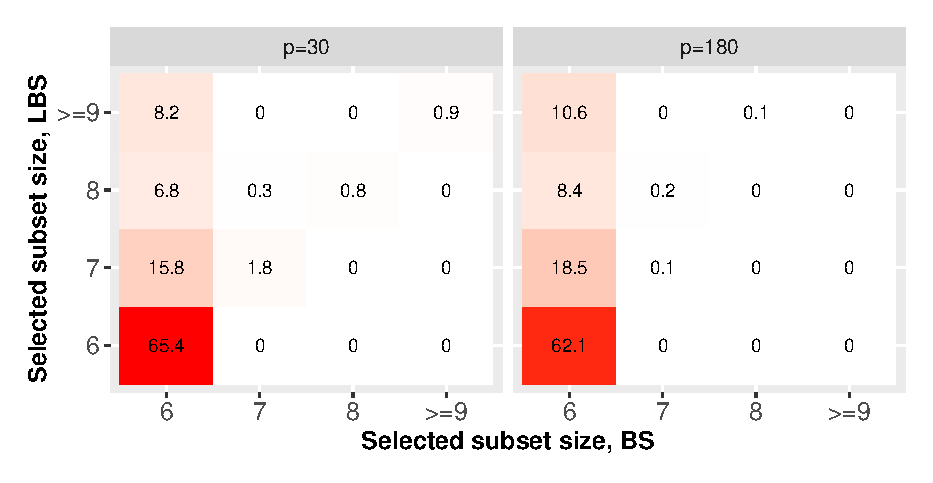
\includegraphics[width=0.9\textwidth]{figures/numvar_bs_lbs.eps}
	\caption{Frequency distributions (in $\%$) of the selected subset size  given by BS and LBS, based on $1000$ replications. The selection rule is C$_p$-edf. The true model is Orth-Sparse-Ex1 with $n=200$, $p_0=6$ and high SNR.}
	\label{fig:numvar_bs_lbs} 
\end{figure}


\iffalse
\begin{figure}[!ht]
	\centering
	\includegraphics[width=0.8\textwidth]{figures/lbs_bs_cp_eg.eps}
	\caption{C$_p$-edf at subset size $k$ for BS and LBS. The true model is Orth-Sparse-Ex1 with $n=200$, $p=180$, $p_0=6$ and high SNR. We assume knowledge of $\mu$ and $\sigma$.}
	\label{fig:lbs_bs_cp_eg} 
\end{figure}
\fi
